\PassOptionsToPackage{dvipsnames}{xcolor}
\documentclass{beamer}
\usepackage[T2A]{fontenc}
\beamertemplatenavigationsymbolsempty
\usecolortheme{beaver}
\setbeamertemplate{blocks}[rounded=true, shadow=true]
\setbeamertemplate{footline}[page number]
% \usepackage[dvipsnames]{xcolor}

\usepackage[utf8]{inputenc}
\usepackage[english,russian]{babel}
\usepackage{amssymb,amsfonts,amsmath,mathtext}
\usepackage{algorithm}
\usepackage{algorithmic}
\makeatletter
\renewcommand{\ALG@name}{Алгоритм}
\makeatother

\DeclareMathOperator*{\argmin}{arg\,min}
\DeclareMathOperator*{\argmax}{arg\,max}

\newtheorem{mytheorem}{Теорема}
\newtheorem{mycorollary}{Следствие}
\newtheorem{myassumption}{Предположение}
\newtheorem{mydefinition}{Определение}


%----------------------------------------------------------------------------------------------------------

\title[\hbox to 56mm{Адаптивное сжатие в распределенной оптимизации}]{Адаптивное сжатие в распределенной оптимизации}
\author[Ф.\,А.~Хафизов]{Фанис Адикович Хафизов\\
\small{Научный руководитель: к.ф.-м.н. А.\,Н.~Безносиков}}
\institute{Кафедра интеллектуальных систем ФПМИ МФТИ\\
Специализация: Интеллектуальный анализ данных\\
Направление: 03.03.01 Прикладные математика и физика}
\date{2024}

%----------------------------------------------------------------------------------------------------------

\begin{document}

%----------------------------------------------------------------------------------------------------------

\begin{frame}

    \maketitle

\end{frame}

%-----------------------------------------------------------------------------------------------------

\begin{frame}{Цель исследования}

    \textbf{Проблема:} Современные нейросети требуют больших вычислительных мощностей, из-за чего приходится прибегать к распределенным методам обучения.

    Одной из главных проблем является скорость передачи данных между устройствами.\\

    $ $\\

    \textbf{Цель:} Предложить новый способ сжатия градиентов для более эффективной коммуникации устройств.\\

    $ $\\

    \textbf{Решение:} Предлагаются семейство смещенных операторов сжатия, использующие показатели важности весов, и схема компенсации ошибок.

\end{frame}

\begin{frame}{Литература}
    \begin{itemize}
        \item Aleksandr Beznosikov, Samuel Horváth, Peter Richtárik, Mher Safaryan. On Biased Compression for Distributed Learning. 2024
        \item Peter Richtárik, Igor Sokolov, Ilyas Fatkhullin. EF21: A New, Simpler, Theoretically Better, and Practically Faster Error Feedback. 2021
    \end{itemize}
\end{frame}

%-----------------------------------------------------------------------------------------------------

\begin{frame}{Постановка задачи}

    Ставится задача распределенной оптимизации.
    \begin{align*}
     \min_{x \in \mathbb{R}^d}\left\{f(x) := \frac{1}{n}\sum\limits_{i = 1}^n f_i(x) \right\},
    \end{align*}
    где $n$~-- количество устройств, $x$~-- обучаемые параметры, $f_i(x)$~-- функция потерь для $i$-го устройства.\\
    $f_i$~-- $\mu$-сильно выпуклая и $L$-гладкая функция.\\
    Требуется сократить количество передаваемой информации, не сильно потеряв в скорости обучения.

\end{frame}

\begin{frame}{Предположения}
    \begin{myassumption}
        Функция $f$ называется $\mu$-сильно выпуклой, если для любых $x, y \in \mathbb{R}^d$ выполняется следующее неравенство:
        \begin{equation}
            f(y) \geq f(x) + \langle \nabla f(x), y - x \rangle + \frac{\mu}{2} \|y - x\|_2^2, \label{eq:strong_convexity}
        \end{equation}
        где $\mu > 0$~--- константа сильной выпуклости.
    \end{myassumption}

    \begin{myassumption}
        Функция $f$ называется $L$-гладкой, если для любых $x, y \in \mathbb{R}^d$ выполняется следующее неравенство:
        \begin{equation}
            \|\nabla f(y) - \nabla f(x)\|_2 \leq L \|y - x\|_2, \label{eq:smoothness}
        \end{equation}
        где $L > 0$~--- константа гладкости.
    \end{myassumption}
\end{frame}

%------------------------------------------------------------

\begin{frame}{Исследуемый метод}
    Для решения задачи распределенной оптимизации используется градиентный спуск со сжатием (DCGD)
    \begin{align*}
     x^{k + 1} = x^k - \frac{\eta}{n} \sum\limits_{i = 1}^n\mathcal{C}_i^k(\nabla f_i(x^k)),
    \end{align*}
    где $\eta$ -- размер шага, $\mathcal{C}_i^k$ -- оператор сжатия на $k$-й итерации $i$-го устройства.\\

    $ $\\
    Для случая одного устройства итерация метода запишется как
    \begin{align*}
     x^{k + 1} = x^k - \eta\mathcal{C}^k(\nabla f(x^k)).
    \end{align*}
\end{frame}

%----------------------------------------------------------------------------------------------------------

\begin{frame}{Предлагаемые операторы сжатия}
    Предлагается определить вектор важности $w \in [0, 1]^d$ и на основе  него построить семейство операторов сжатия $\mathcal{C}(x, w)$.\\
    $ $\\
    Для нахождения вектора $w$ решается задача оптимизации
    \begin{align*}
     w^k = \argmin_{w \in Q} f(x^k - \eta w \odot \nabla f(x^k)),
    \end{align*}
    где $Q$ -- ограниченное множество, $\odot$ -- поэлементное умножение.\\

    В качестве $Q$ рассмотрены следующие варианты:
    \begin{itemize}
        \item $\Delta_{d - 1} = \{x \in \mathbb{R}^d ~|~ \|x\|_1 = d, x_i \geq 0, i = \overline{1, d}\}$~--- симплекс размерности $d - 1$;
        \item $[a, b]^d$~--- куб со сторонами длиной $b - a$.
    \end{itemize}
\end{frame}

%----------------------------------------------------------------------------------------------------------

\begin{frame}{Примеры операторов сжатия с важностью}
    \begin{itemize}
        \item \textbf{Важностное прореживание}.\\
        \begin{equation}
            \mathcal{C}(\nabla f(x)) = \sum_{i=1}^k \nabla_{(i)} f(x) e_{(i)},
        \end{equation}
        где координаты расположены по убыванию значений важности $w_{(1)} \geq w_{(2)} \geq \dots \geq w_{(d)}$.
        \item \textbf{Рандомизированное важностное прореживание}\\
        \begin{equation}
            \mathcal{C}(\nabla f(x)) = \sum_{i \in S} \nabla_i f(x) e_i,
        \end{equation}
        где $S$~--- множество индексов, выбранных случайно с вероятностью, пропорциональной значениям важности $w$.
    \end{itemize}
\end{frame}

\begin{frame}{Примеры операторов сжатия с важностью}
    \begin{itemize}
        \item \textbf{Важностное прореживание с перевзвешиванием}\\
        \begin{equation}
            \mathcal{C}(\nabla f(x)) = \sum_{i=1}^k w_{(i)} \nabla_{(i)} f(x) e_{(i)},
        \end{equation}
        где координаты расположены по убыванию значений $|w_{(1)} \nabla_{(1)} f(x)| \geq \dots \geq |w_{(d)} \nabla_{(d)} f(x)|$.
        \item \textbf{Рандомизированное важностное прореживание с перевзвешиванием}\\
        \begin{equation}
            \mathcal{C}(\nabla f(x)) = \sum_{i \in S} w_i \nabla_i f(x) e_i,
        \end{equation}
        где $S$~--- множество индексов, выбранных случайно с вероятностью, пропорциональной значениям важности $w$.
    \end{itemize}
\end{frame}

%----------------------------------------------------------------------------------------------------------

\begin{frame}{Сходимость DCGD с оператором $ImpK$}
    \begin{mytheorem}[Хафизов Ф.\,А., 2025]
        Пусть $Q = [1, 2]^d, \gamma \leq \frac{2}{L}$. Тогда
        \begin{equation}
            f(x^T) - f^* \leq \left(1 - 2\mu \gamma \left(\frac{k}{d} - 2 L \gamma\right)\right)^T (f(x^0) - f^*).
        \end{equation}
    \end{mytheorem}
    \begin{mycorollary}
        При выборе $\gamma = \frac{k}{4dL}$ для достижения точности $\varepsilon > 0$ по функции требуется
        \begin{equation}
            T \geq \frac{4L}{\mu} \left(\frac{d}{k}\right)^2 \log\left(\frac{f(x^0) - f^*}{\varepsilon}\right)
        \end{equation}
        итераций.
    \end{mycorollary}
\end{frame}

\begin{frame}{Схема компенсации ошибок SCAM}
    \begin{algorithm}[H]
        \caption{SCAM (Одно устройство)}
        \label{alg:scam_single}
        \begin{algorithmic}
            \STATE {\bf Ввод:} стартовая точка $x^0$, шаг обучения $\gamma$, количество итераций $T$, начальная ошибка $\varepsilon^0 = 0$.
            \FOR{$t = 0, 1, \ldots, T - 1$}
                \STATE $g^t = \nabla f(x^t)$
                \STATE $c = \mathcal{C}^t (\varepsilon^t + g^t)$
                \STATE $\tilde{g}^t = \mathcal{C}^t \left(\sum\limits_{i=1}^{d} I\{c_i \neq 0\} g^t_i e_i\right)$
                \STATE $\varepsilon^t = \varepsilon^{t-1} + g^t - \tilde{g}^t$\\
                \STATE $x^{t+1} = x^t - \gamma \tilde{g}^t$
            \ENDFOR
            \STATE {\bf Вывод:} $x^k$
        \end{algorithmic}
    \end{algorithm}
    
\end{frame}



\begin{frame}{Сходимость SCAM с оператором $TopK$}
    \begin{myassumption}\label{prop:scam_single_partial_norm}
        В схеме SCAM $TopK$ частично сохраняет норму градиента:
        \begin{equation}
            \|\tilde{g}^t\|_2^2 \geq \delta \|g^t\|_2^2.
        \end{equation}
    \end{myassumption}
    \begin{mytheorem}[Хафизов Ф.\,А., 2025]
        Пусть $\gamma \leq \frac{2}{L}$. Тогда для любого $T \geq 1$ верно:
        \begin{equation}
            f(x^T) - f^* \leq (1 - \mu \gamma (2 - L \gamma) \delta)^T (f(x^0) - f^*).
        \end{equation}
    \end{mytheorem}
    \begin{mycorollary}
        Пусть выбрано значение шага $\gamma = \frac{1}{L}, \delta \simeq \frac{k}{d}$. Тогда для достижения точности $\varepsilon > 0$ по функции требуется
        \begin{equation}
            T \simeq \frac{L d}{\mu k} \log\left(\frac{f(x^0) - f^*}{\varepsilon}\right).
        \end{equation}
        итераций.
    \end{mycorollary}
\end{frame}

\begin{frame}{Эксперимент. Классификация изображений}

    \begin{figure}[ht]
        \centering
        \begin{minipage}{0.4\textwidth}
            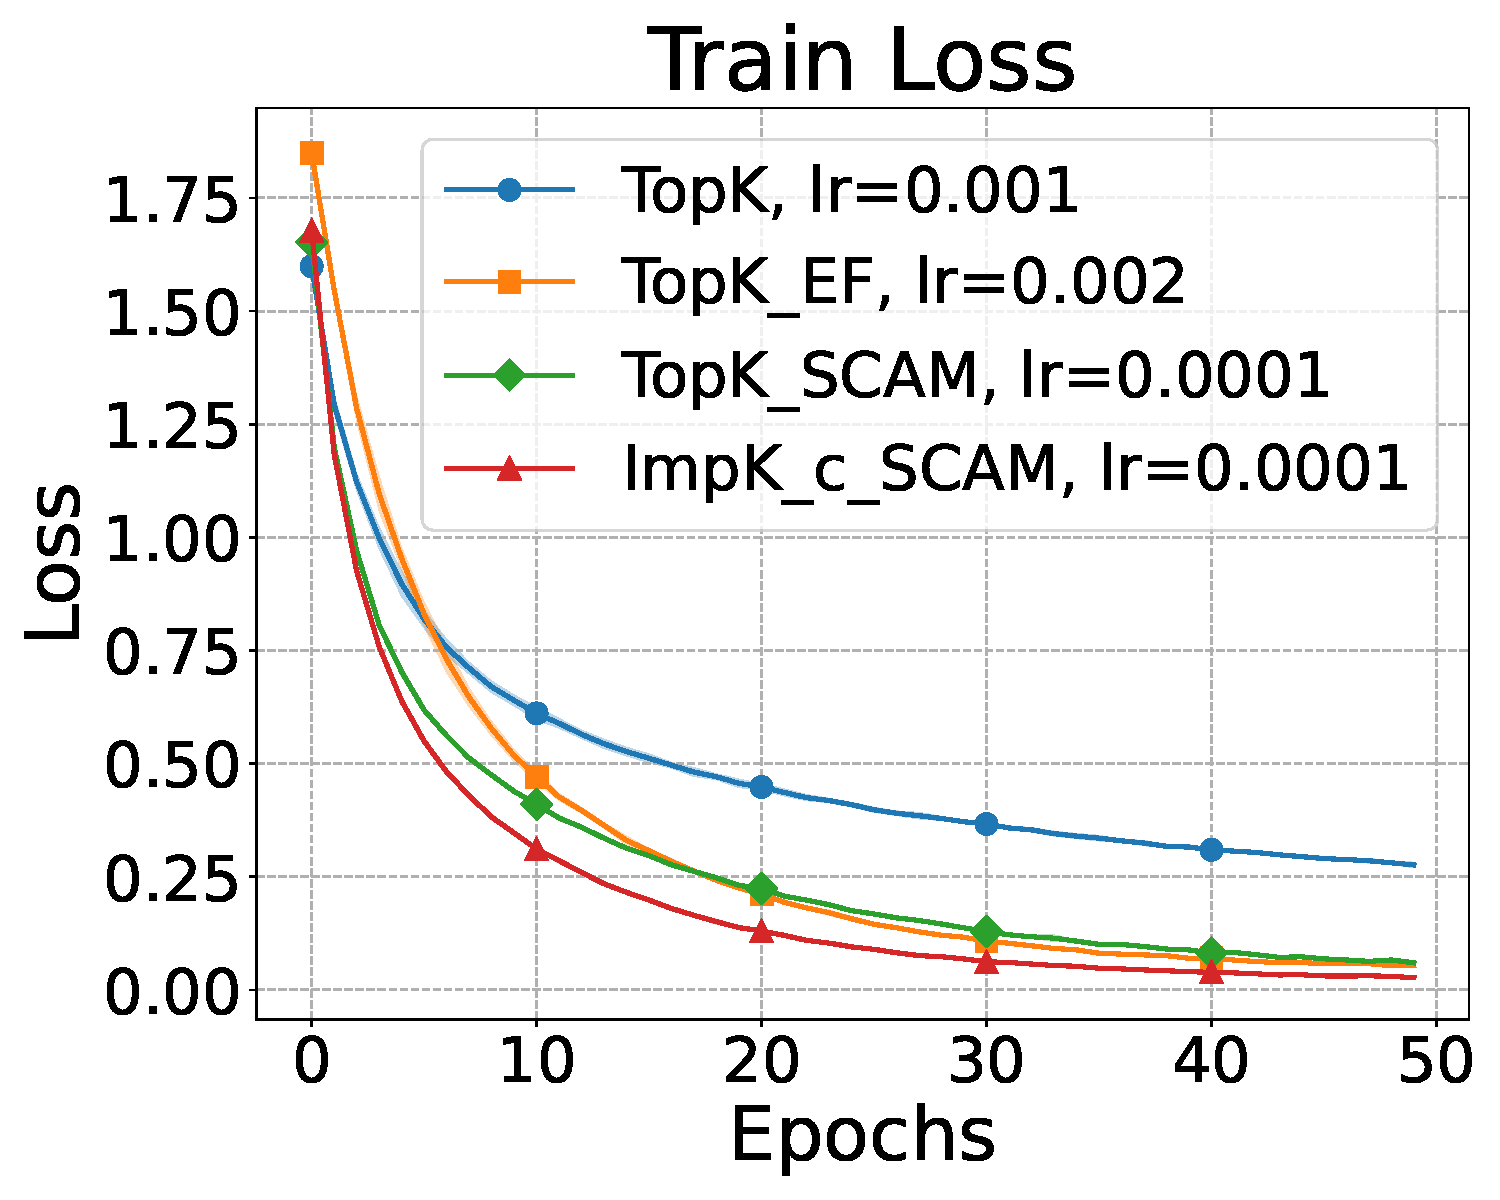
\includegraphics[width=\textwidth]{../paper/figures/resnet/experiment2/Train Loss.pdf}
        \end{minipage}
        \begin{minipage}{0.4\textwidth}
            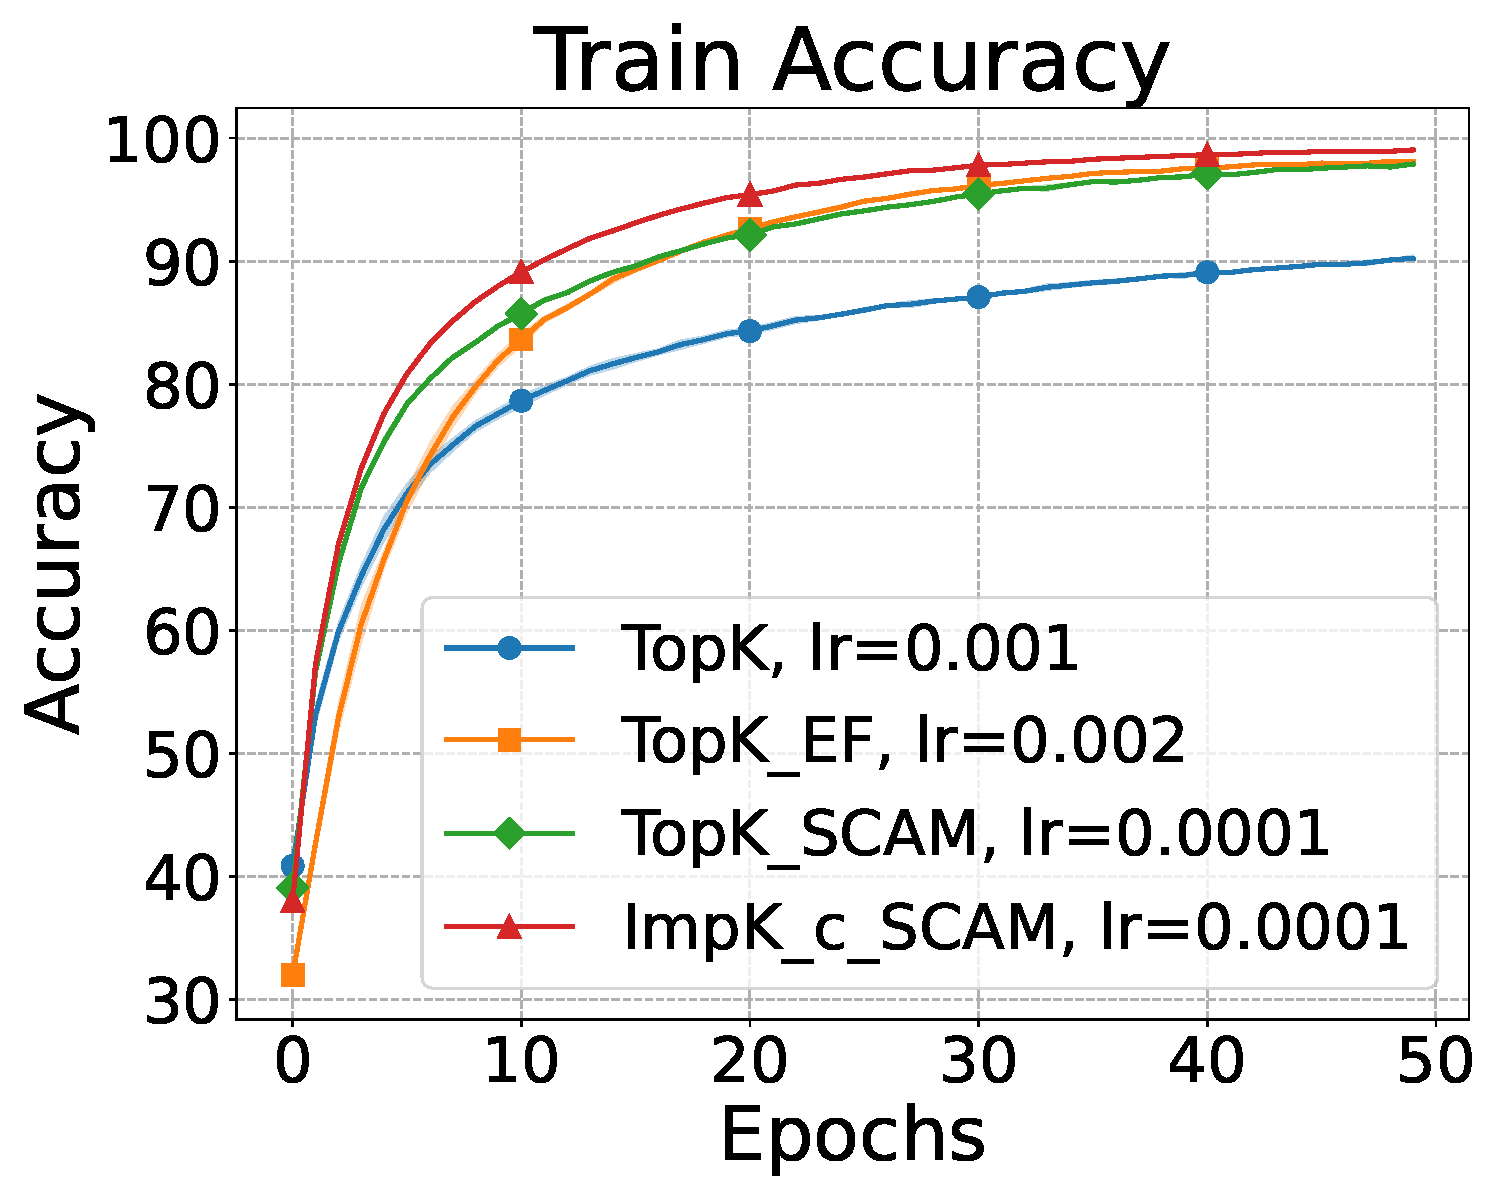
\includegraphics[width=\textwidth]{../paper/figures/resnet/experiment2/Train Accuracy.pdf}
        \end{minipage}
        \begin{minipage}{0.4\textwidth}
            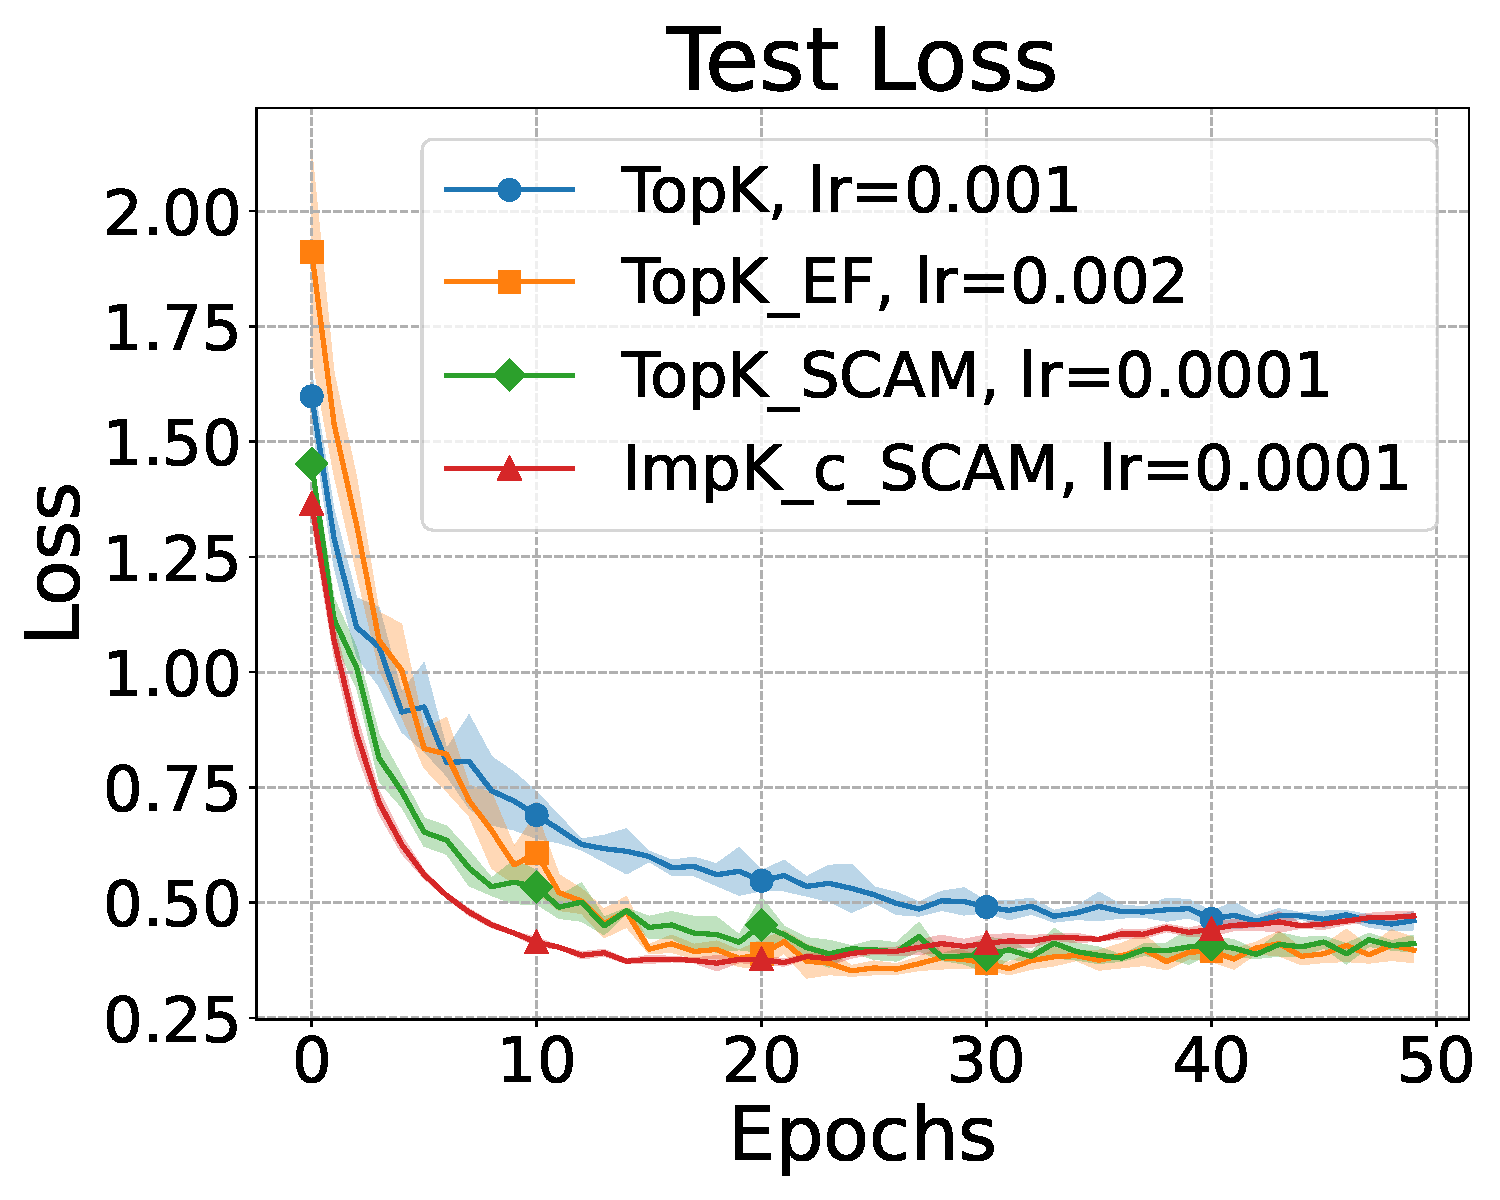
\includegraphics[width=\textwidth]{../paper/figures/resnet/experiment2/Test Loss.pdf}
        \end{minipage}
        \begin{minipage}{0.4\textwidth}
            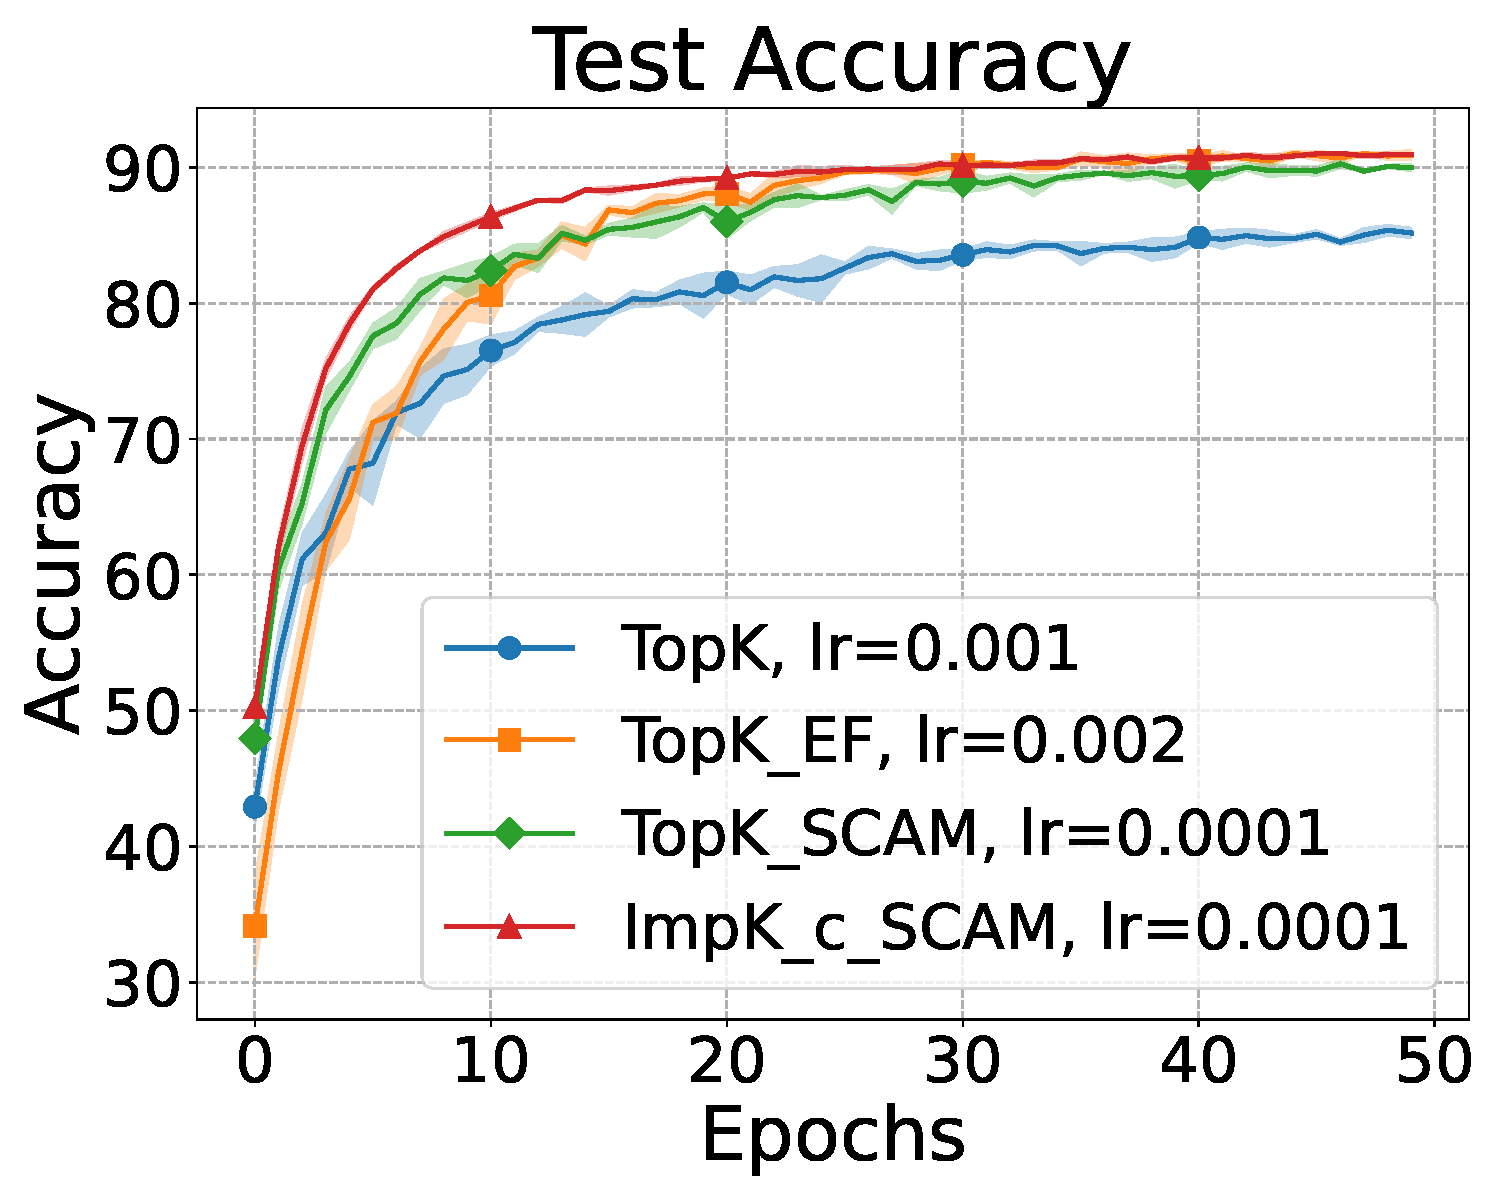
\includegraphics[width=\textwidth]{../paper/figures/resnet/experiment2/Test Accuracy.pdf}
        \end{minipage}
        \caption{Сравнение сходимости предложенного метода SCAM с $ImpK_c$ и вариациями $TopK$ в процессе обучения ResNet-18 на CIFAR-10.}
    \end{figure}

\end{frame}

%----------------------------------------------------------------------------------------------------------

\begin{frame}{Эксперимент. Трансформерная архитектура}

    \begin{figure}[ht]
        \centering
        \begin{minipage}{0.4\textwidth}
            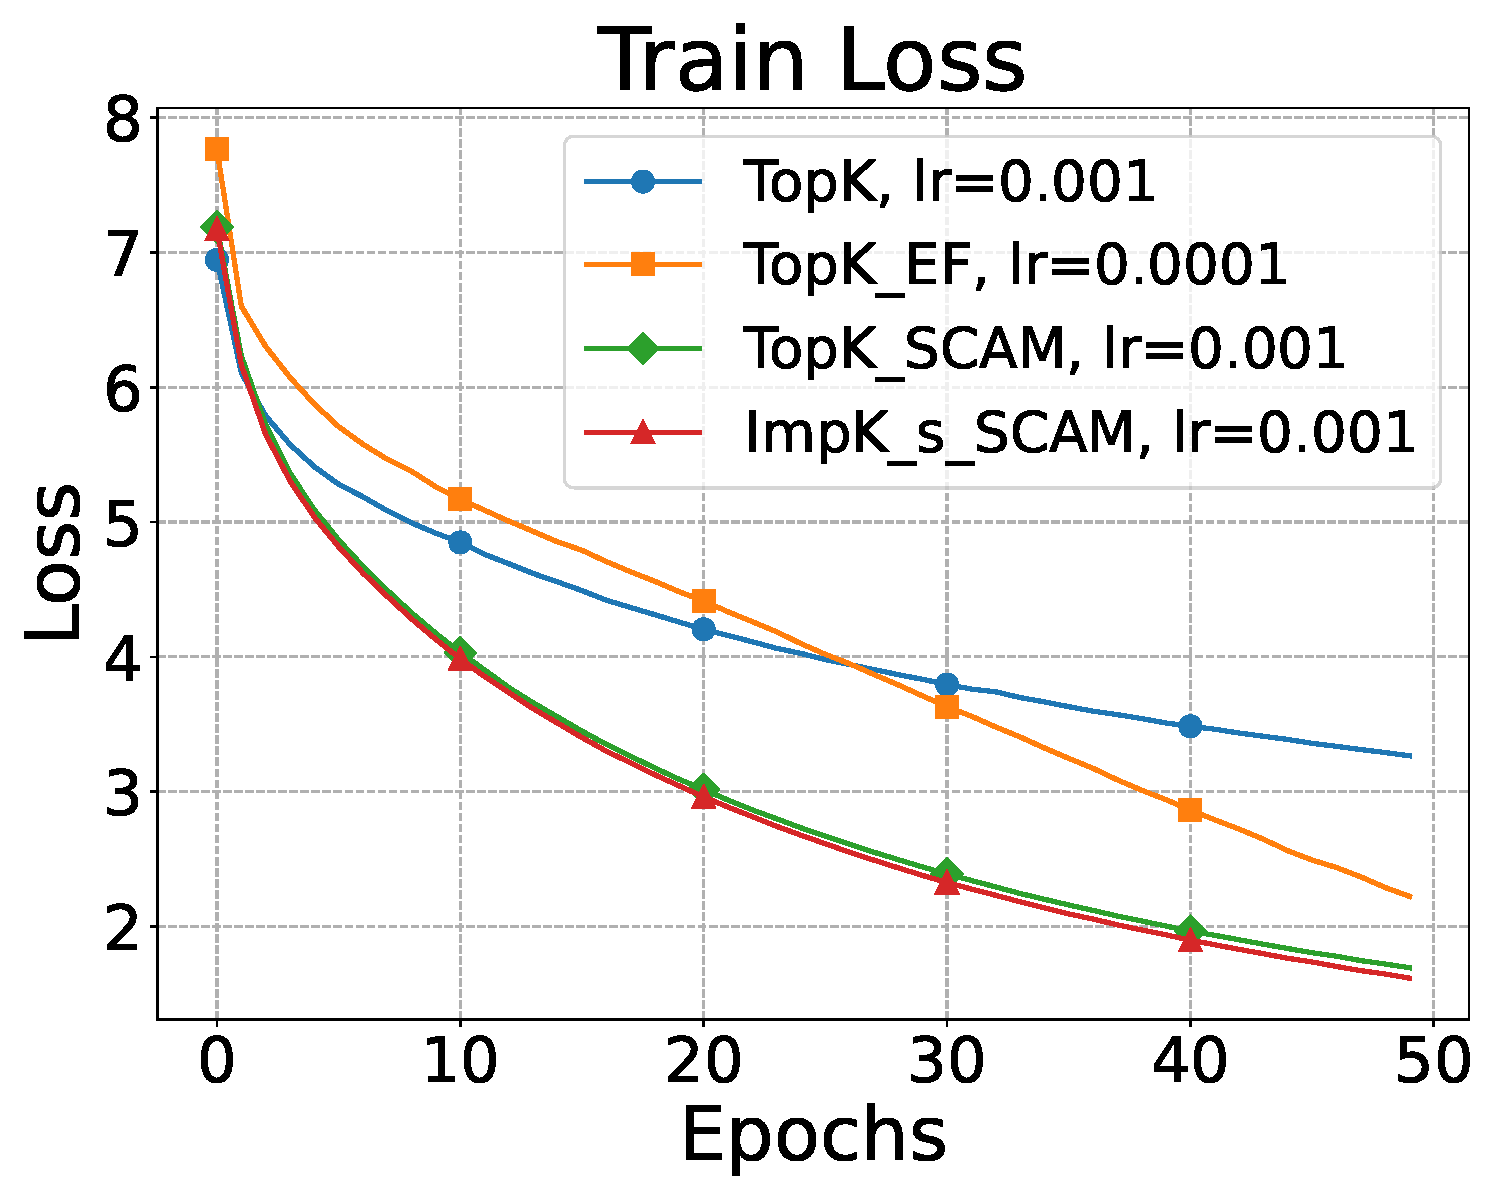
\includegraphics[width=\textwidth]{../paper/figures/gpt2/experiment2/Train Loss.pdf}
        \end{minipage}
        \begin{minipage}{0.4\textwidth}
            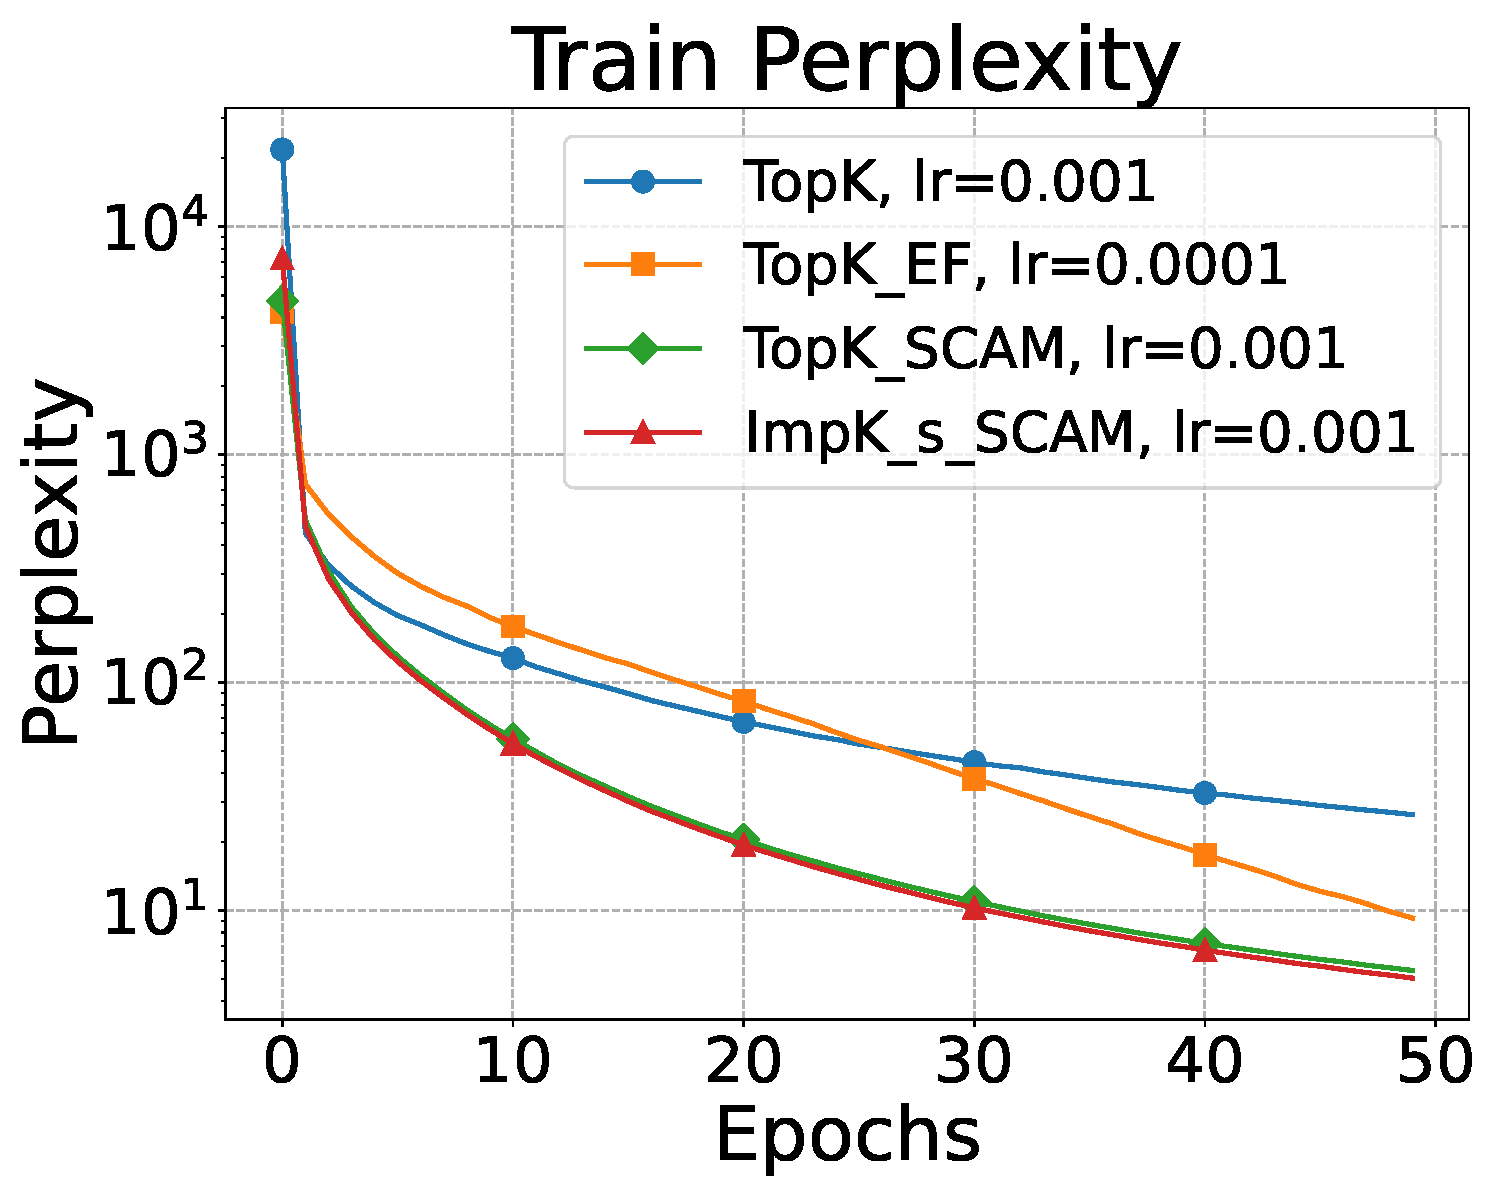
\includegraphics[width=\textwidth]{../paper/figures/gpt2/experiment2/Train Perplexity.pdf}
        \end{minipage}
        \begin{minipage}{0.4\textwidth}
            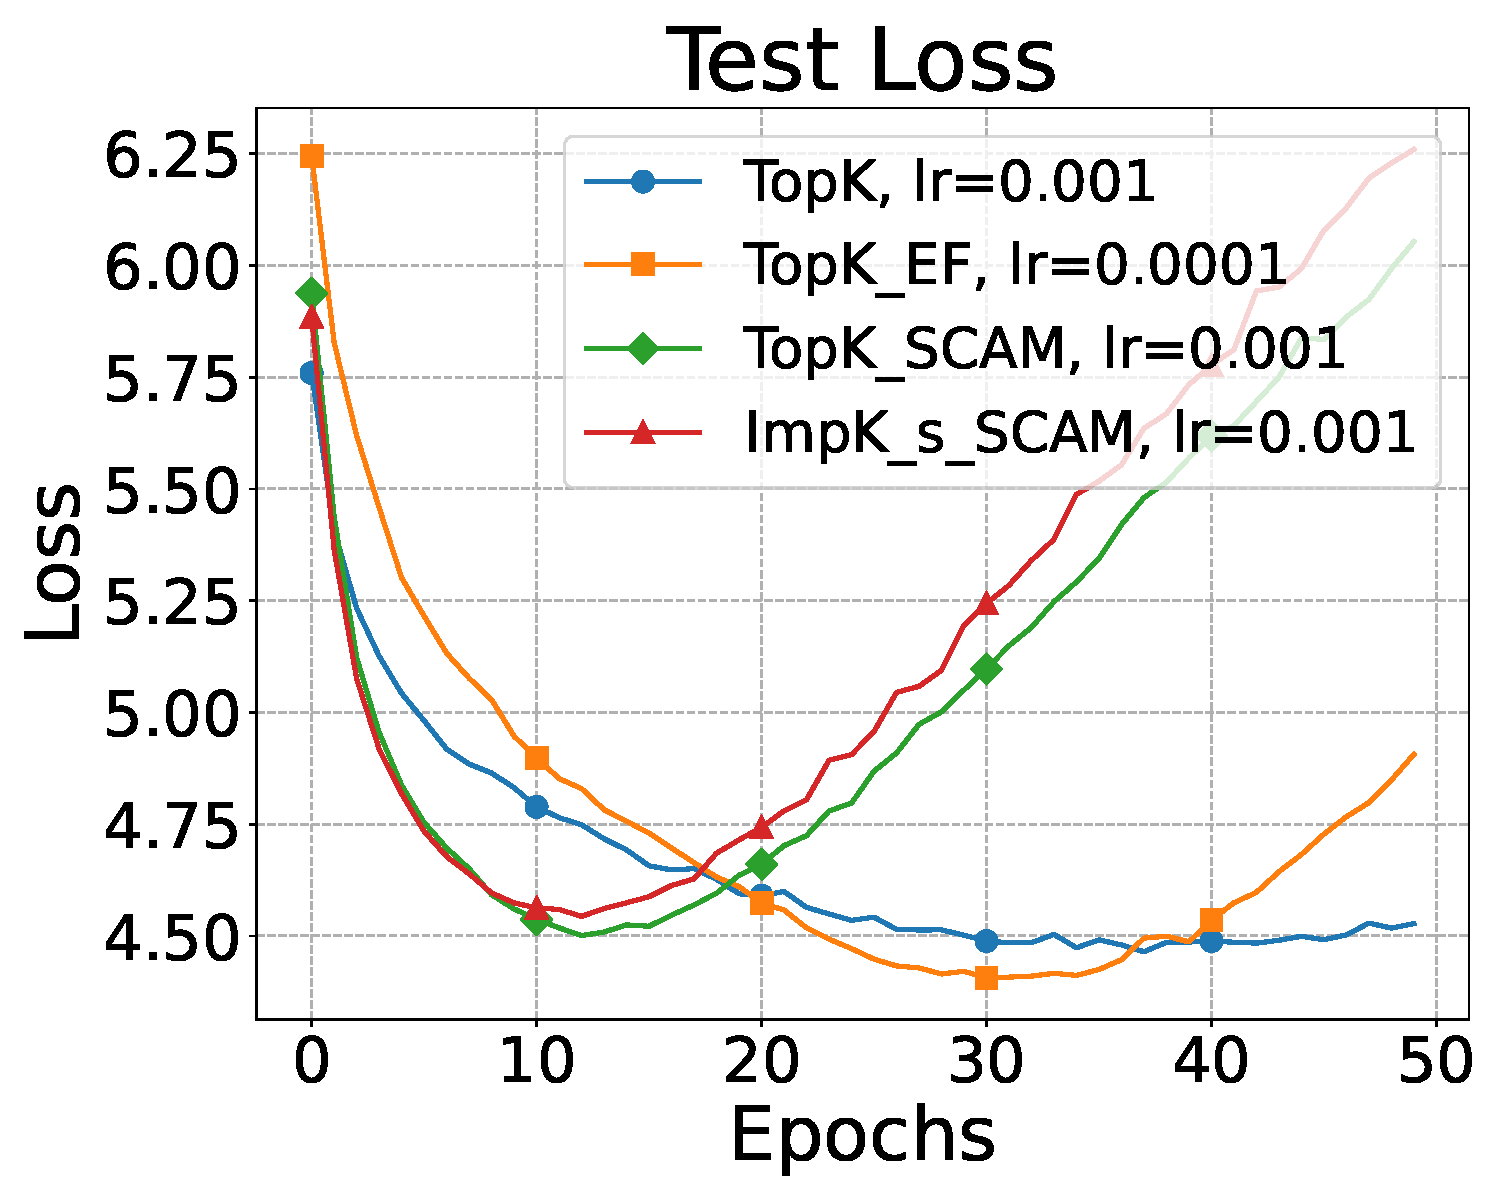
\includegraphics[width=\textwidth]{../paper/figures/gpt2/experiment2/Test Loss.pdf}
        \end{minipage}
        \begin{minipage}{0.4\textwidth}
            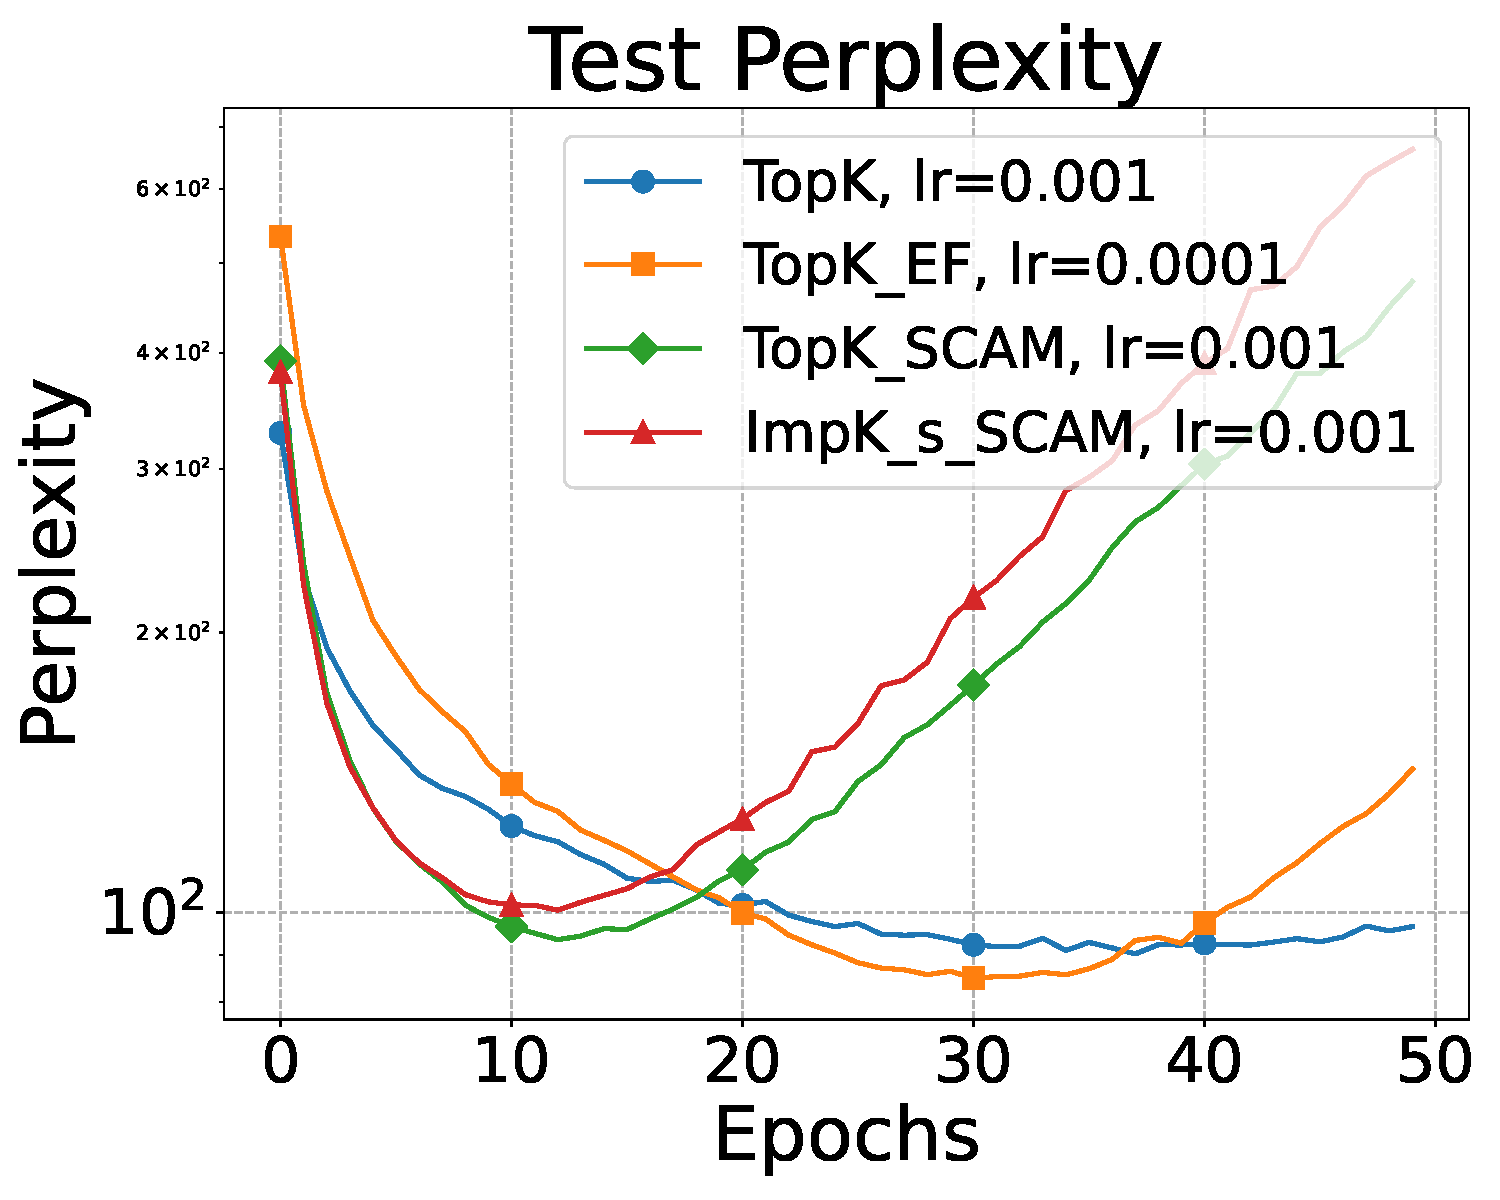
\includegraphics[width=\textwidth]{../paper/figures/gpt2/experiment2/Test Perplexity.pdf}
        \end{minipage}
        \caption{Сравнение сходимости предложенного метода SCAM с $ImpK_s$ и вариациями $TopK$ в процессе обучения GPT-2 на WikiText2.}
    \end{figure}

\end{frame}

%----------------------------------------------------------------------------------------------------------

\begin{frame}{Заключение}
    \begin{block}{Выносится на защиту}
    \begin{enumerate}
        \item Предложено семейство операторов сжатия, использующие вектор важности.
        \item Для одного оператора сжатия по важности получена оценка сходимости.
        \item Предложена схема компенсации ошибки SCAM.
        \item Получена теоретическая оценка сходимости для SCAM с оператором $TopK$.
        \item Вычислительные эксперименты показали превосходство схемы SCAM с $ImpK$ над остальными методами.
    \end{enumerate}
    \end{block}

\end{frame}

%----------------------------------------------------------------------------------------------------------

\end{document}
